% Crucial Preamble
\documentclass[12pt,letterpaper]{article} \usepackage{amsmath} \usepackage{graphicx} \usepackage[margin=1in]{geometry} \usepackage{longtable}  \usepackage{amssymb}

% Extra Preamble
\usepackage{fancyhdr} \usepackage{enumitem} \usepackage{float} \usepackage{soul}
\usepackage{multicol} \usepackage[compact]{titlesec}


% frames with display breaks
\usepackage{mdframed}
\allowdisplaybreaks

% change spacing
\usepackage{setspace}
\setlength{\parskip}{0.4\baselineskip}

% Remove paragraph indentation
\setlength{\parindent}{0pt}

% Reduce space before and after section headings
%\titlespacing*{\section}{0pt}{0.1\baselineskip}{0.2\baselineskip}

% changes font
%\renewcommand{\familydefault}{\sfdefault}

% adds header and footer
\pagestyle{fancy}
\fancyhead{} \fancyhead[C]{PHY 2323 Summary Sheet} \fancyhead[L]{PHY2323} \fancyhead[R]{Owen Daigle}
\fancyfoot{} \fancyfoot[C]{\thepage}


\begin{document}
	
	\begin{center}
		\Large\textbf{PHY 2323 Summary Sheet} \\
		\vspace{0.5em}
	\end{center}
	
	\section{Math Introduction}
	There are 3 main coordinate systems:
	\begin{enumerate}[]
		\item Cartesian ($x,y,z$)
		\item Cylindrical ($\rho, \phi, z$)
		\item Spherical ($r,\phi, \theta$)
	\end{enumerate}

	We have a few charts to help us convert between the systems:
	\begin{center}
		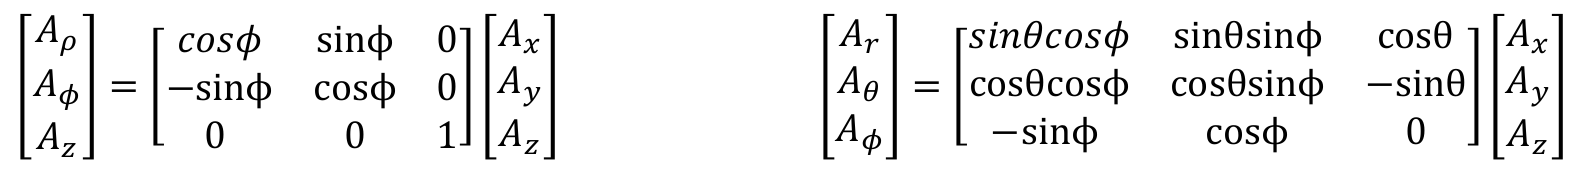
\includegraphics[width=0.8\linewidth]{trans}
	\end{center}

	When integrating, the differential line/surface/volume elements can be found in the following chart:
	\begin{center}
		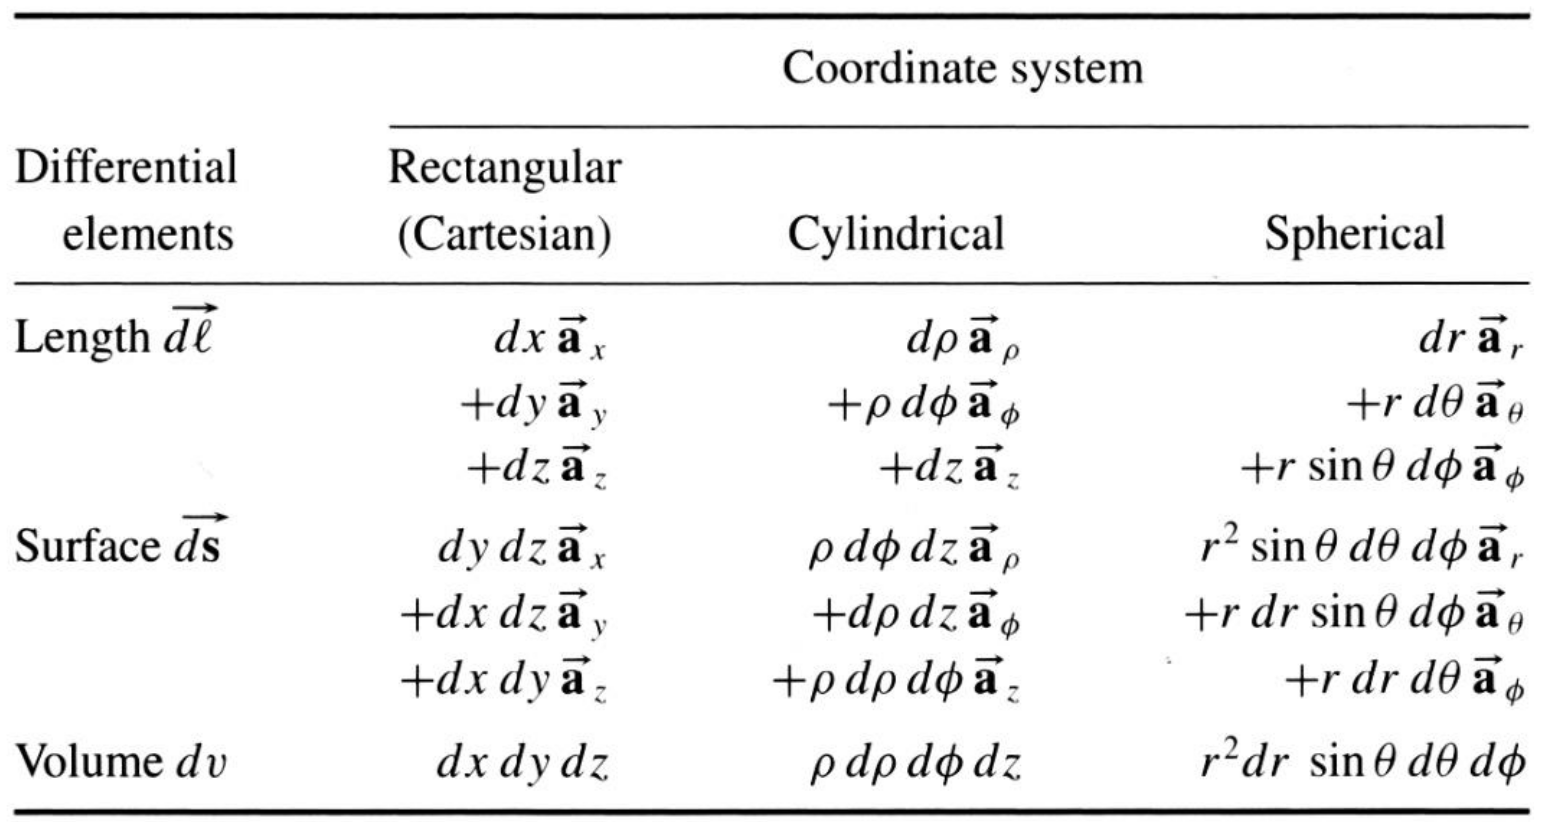
\includegraphics[width=0.7\linewidth]{differential_surfaces}
	\end{center}
	
	Tables taken from PHY2323 Course Formula Sheet.
	
	\section{Electric Fields}
	We have 2 ways to talk about electric fields. There is the \textbf{Electric Field} $\vec E$, and the \textbf{Elecric Flux Density }$\vec D$.
	\begin{align*}
		\vec D = \epsilon \vec E
	\end{align*}
	
	\subsection{Coulombs Law}
	Coulomb's law is used to sum up all the charges in a location which will give an electric field $E$.
	\begin{align*}
		\vec E (\vec r) = \frac{1}{4\pi \epsilon_0} \int_S \frac{\rho(\vec r\prime)(\vec r - \vec r\prime)}{|\vec r - \vec r\prime | ^3}\mathrm d l
	\end{align*}
	This can also be extended to a surface with $\mathrm ds$ and 2 integrals, or volume with $\mathrm dv$
	
	Note that anything with the $\prime$ means that it is related to the \textbf{surface of charge}, and anything without the prime is related to the \textbf{observation point.}
	
	\begin{mdframed}
		\textbf{Ex. }
	\end{mdframed}
	
	\subsection{Gausses Law}
	Gausses Law is basically a shorter way of finding the $\vec E$ field rather than using Coulomb's equation. It works well when there is \textbf{symmetry}.
	
	It can be used on a \textbf{closed surface} where we make a guassian surface (such as a sphere, or cylander) at the point of interest. 
	\begin{align*}
		\int_S \vec E \mathrm d \vec s = \frac{Q_{enc}}{\epsilon}
	\end{align*}

	We also have the $\vec D$ field which is the \textit{Electric Flux Density}.
	\begin{align*}
		\int_S \vec D \mathrm d \vec s = Q_{enc}
	\end{align*}
	
	Finally, we have the flux $\psi$, a scalar. 
	\begin{align*}
		\psi = \epsilon \int_s \vec E \mathrm d \vec s = \int \vec D \mathrm d \vec s
	\end{align*}

	This is useful in 3 main cases. 
	\begin{enumerate}[]
		\item Spherical Symmetry is present
		\item Cylindrical symmetry is present (long line of charge with uniform $\rho$ or cylander with no angular dependance)
		\item Planar Symmetry (Long 2D surface of charge)
	\end{enumerate}

	A useful piece of information is if we want to find the $Q_{enc}$, we can often just integrate the charge density in a volume $V$ (or surface $S$).
	\begin{align*}
		Q_{enc} = \iiint_V \rho \mathrm d V
	\end{align*}

	Also, the $\vec D$ field is just the $\vec E$ field times a factor of $\epsilon$ ($\vec D = \epsilon \vec E$) 
	
	\begin{mdframed}
		\textbf{Ex. }
	\end{mdframed}
	
	\subsection{Energy Stored in an Electric Field}
	We say that $W$ is the energy stored in an electric field, or the \textbf{energy required to assemble a charge distribution}. 
	
	We can calculate this by summing up the product of the charge density and potential difference across a line/surface/volume.
	\begin{align*}
		W = \frac{1}{2}\int_{S\prime}\rho_s(\vec r\prime)*V(\vec r\prime) \mathrm d v\prime
	\end{align*}
	
	\section{Electric Potential}
	This is the potential energy per unit charge. AKA the voltage. This is a \textbf{scalar field}. This is \textit{independant of the path chosen}. 
	\begin{align*}
		V(\vec r) = \frac{1}{4\pi \epsilon _0} \int_{l\prime }\frac{\rho _l \mathrm d l\prime}{|\vec r-\vec r\prime| }
	\end{align*}
	This can be extended into 2d or 3d space by changing the $l\prime$ and $\mathrm d l\prime$ for $s\prime, \mathrm d s\prime$ or $v\prime, \mathrm d v\prime$.
	
	Then we can relate the change in voltage to the electric field:
	\begin{align*}
		\vec E = -\nabla V \qquad \nabla V = -\int \vec E\cdot \mathrm d \vec l
	\end{align*}
	
	\begin{mdframed}
		\textbf{Ex. }
	\end{mdframed}

	\subsection{Electric Dipole}
	A \textbf{dipole} is a pair of equal and opposite charges that are very close to each other relative to the point of observation.
	
	This means that at the point of observation, they \textbf{seem} as though they are only one charge. 
	
	We have an equation that relates the charge of each end of the dipole $q$, the distance between the charges $d$, and the vector between the dipole and the observation point $\vec r$. This vector must be large compared to $d$.
	\begin{align*}
		V(\vec r) = \frac{(qd) \hat z \cdot \hat r}{4\pi \epsilon |r|^2}
	\end{align*}

	\subsection{Capacitors}
	The \textbf{capacitence} $C$ can be calculated using the following formula:
	\begin{align*}
		C=\frac{Q}{\Delta V}
	\end{align*}
	In practice, we use the following 3 step procedure:
	\begin{enumerate}[noitemsep]
		\item Find $E$
		\item Find $\Delta V$
		\item Find $C$ using $C=\frac{Q}{\Delta V} $
	\end{enumerate}

	\begin{mdframed}
		\textbf{Ex. }
	\end{mdframed}
	
	\section{Materials in Electric Fields}
	There are 3 types of materials:
	\begin{enumerate}[]
		\item Conductors
		\item Insulators
		\item Semiconductors
	\end{enumerate}

	We have rules concerning the \textbf{normal} and \textbf{tangential} part of the boundary between 2 materials, so we need to break up the field into those two components. 
	
	\begin{center}
		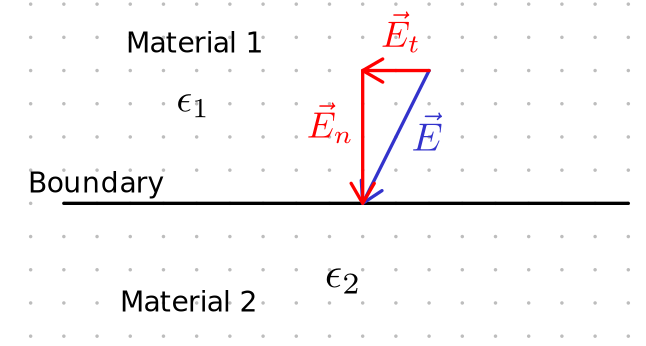
\includegraphics[width=0.55\linewidth]{../MAT2377/boundary-conditions-E}
	\end{center}
	
	
	To obtain the \textbf{normal direction}, we take the unit vector of the boundary, and this is our normal unit vector ($\hat n = \frac{\vec n}{|n|}$).
	
	If we then want to get the \textbf{normal part} of $E$, we dot product it with $\hat n$, then append $n$ to keep direction ($\vec E_n = (\vec E\cdot \hat n)\hat n$)
	
	The \textbf{tangential part }is just $\vec E_t = \vec E - \vec E_n$

	\subsection{Boundary between 2 Dielectrics}
	If we have 2 electric fields between 2 \textbf{dielectric} (insulators) surfaces, we have the following formulas for the bounds:
	\begin{align*}
		E_{1t} = E_{2t} \qquad \epsilon_1E_{1n}-\epsilon_2 E_{2n} = \rho_s
	\end{align*}

	\subsection{Surface of a Conductor}
	If we have an electric field at the \textbf{surface }of a \textbf{conductive} surface (note that inside the surface $E=0$), we have the following formulas for the bounds:
	\begin{align*}
		E_{1t} = E_{2t} = 0 \qquad E_{n} = \frac{\rho_s}{\epsilon_0}
	\end{align*}

	\begin{mdframed}
		\textbf{Ex. }
	\end{mdframed}

	\section{Laplace and Poisson Equations}
	These equations will give us a \textbf{general form of the equation} for the solution, and then using \textbf{2 conditions} (such as points) we can sub them into the form of the equation and solve the equation. 
	
	The whole laplacian equation is very complicated, but we have 2 special cases of note:
	\begin{align*}
		\nabla^2 V = \frac{-\rho_v}{\epsilon} \qquad \text{ or if no charge density (charges on surface): } \nabla^2V=0
	\end{align*}

	\begin{mdframed}
		\textbf{Ex. } As a very general example, if we want to find the voltage in a conductor (charges just on surface)
		
		We start by using the laplace equation:
		\begin{align*}
			\nabla^2 V = 0 \implies \frac{\partial^2 V}{\partial x^2} + \frac{\partial^2 V}{\partial y^2} + \frac{\partial^2 V}{\partial z^2} = 0
		\end{align*}
		\textit{For simplicity, I will consider a situation where the V only exists in the $z$ direction, hence the $x$ and $y$ components will be 0.}
		\begin{align*}
			\frac{\partial^2 V}{\partial z^2} = 0
		\end{align*}
		Since $\frac{\partial^2 V}{\partial z^2}=0$, then we must say that $\frac{\partial V}{\partial z} = a$ where $a$ is a constant. We must then say that $V = az+b$ where $a$ and $b$ are constants.
		
		This is because integrating $\frac{\partial^2 V}{\partial z^2}=0$ once gives us $\frac{\partial V}{\partial z}=a$ and then $a$ second time gives $V=az+b$
		
		Then we must have some boundary conditions given such as when $z=0$, $V=0$, and when $z=1$, $V=5$. Then we can sub in and solve for $a$ and $b$.
		
		Then we have $V$ at any point.
	\end{mdframed}

	We can also do this for spherical or cylindrical coordinates, except for the laplacian ($\nabla^2$) is different.
	
	\section{Currents}
	Current is just the rate of which charge travels with respect to time. Measured in either $\frac{C}{s}$ or $A$.
	
	By definition, the current density is just the \textbf{amount of current} passing through a \textbf{cross sectional area}. Note that this does NOT include parallel current since this current does not actually traverse \textbf{through} the cross sectional area.
	\begin{align*}
		\vec J=\frac{I}{A} \qquad I = \int_S \vec J \cdot \mathrm d \vec s
	\end{align*}

	\begin{center}
		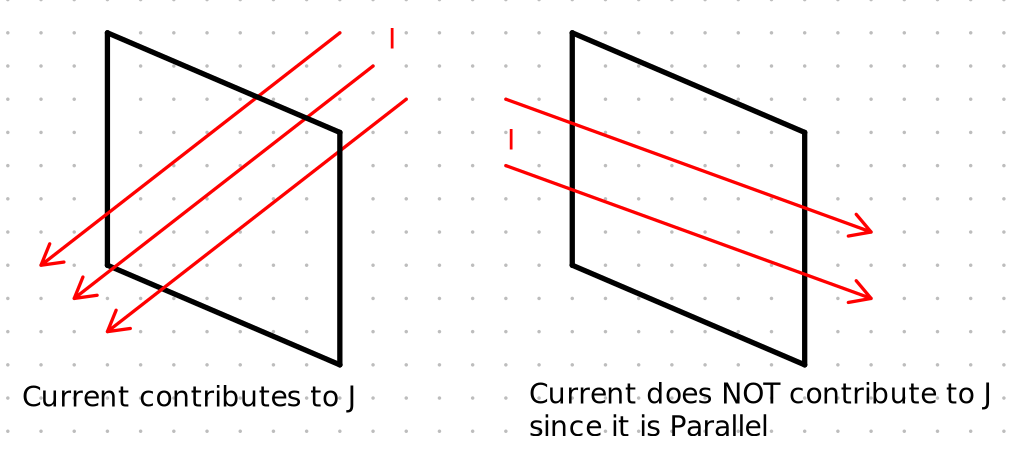
\includegraphics[width=0.7\linewidth]{../MAT2377/current-density-contirbutions}
	\end{center}


	\subsection{Resistance}
	Resistance is defined as:
	\begin{align*}
		R = \frac{L}{\sigma A} = \frac{\rho L}{A}
	\end{align*}
	These are equivalent since $\sigma = \rho^{-1}$ where $\rho$ is the \textbf{resistivity}, and $\sigma$ is the \textbf{conductivity}.
	
	Those equations work fine for a single area, but if we need to sum up the areas, we have 2 techniques. The first is just by summing up the above equation using an integral. The second is based on Ohms law. 
	\begin{align*}
		 &R = \frac{L}{\sigma A} = \int_l \frac{\mathrm d \vec l}{\iint_S \sigma \mathrm d \vec s} &R = \frac{\Delta V}{I} = \frac{-\int_l \vec E \cdot \mathrm d \vec l}{\int_S \vec J \cdot \mathrm d \vec s} 
	\end{align*}

	\begin{mdframed}
		\textbf{Ex. } We have a long cable (length = L) made of 2 materials. The inner one is copper, and the outer one is aluminium. They have outer radius of $r_o$ and inner radius of $r_i$. It carries current I. We want to find the resistance. 
		
		First we can draw a diagram of the situation. 
		\begin{center}
			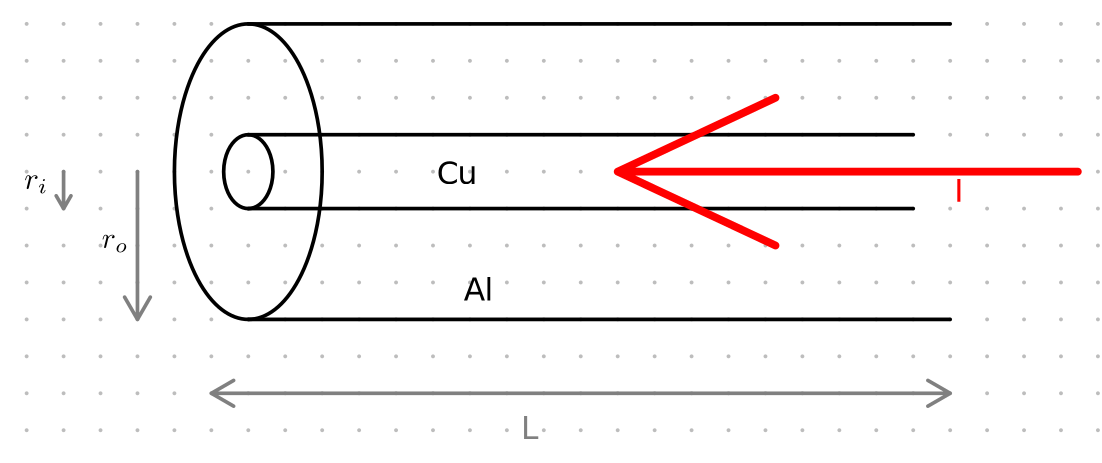
\includegraphics[width=0.6\linewidth]{ex}
		\end{center}
		We will break this up into cross sectional disks, and then sum them all up along the length. I need to do this for each material. For the outer material Al, I need to subtract the inner part since that does not exist. Then we can add up both materials (Al + Cu).
		\begin{align*}
			R_{Cu} = \int_l \frac{\mathrm d \vec l}{\iint_s \sigma \mathrm d \vec s} = \int_0^L \frac{\mathrm d l}{\sigma_{cu}\pi r_i^2} = \frac{L}{\sigma_{cu}\pi r_i^2}
		\end{align*}
		We do not really have to do the bottom integral since the density is constant, and each slice has the same area of $\pi r^2$. However if we wanted to, we could take the integral of the disk to get $\int_0^{2\pi}\int_0^{r_i} \rho \mathrm d \rho \mathrm d \phi = 2\pi \left(\frac{\rho^2}{2}\right)^{r_i}_0=\pi r_i^2$
		
		To get the resistance for the Al part, we need to integrate both the radius from 0 to $r_o$, and from 0 to $r_i$, and then subtract the inner component. 
		\begin{align*}
			R_{Al} = \int_0^L \frac{\mathrm d l}{\sigma_{Al}\pi r_o^2} - \int_0^L \frac{\mathrm d l}{\sigma_{Al}\pi r_i^2} = \frac{L}{\sigma_{Al}\pi (r_o^2-r_i^2)}
		\end{align*}
		Then the entire resistance would be the inverse sum of both of thse since they are in parallel. 
		\begin{align*}
			R_{tot} = \frac{1}{\frac{1}{R_{Al}}+\frac{1}{R_{Cu}}}
		\end{align*}
		If we want the current say through the Cu part, we can just use a current dividor by doing:
		\begin{align*}
			I_{Cu} = I\cdot \frac{R_{Al}}{R_{Al}+R_{Cu}}
		\end{align*}
		If we want the current density through this Copper part, we just do the current over the area:
		\begin{align*}
			J_{Cu} = \frac{I}{A} = \frac{I_{Cu}}{\pi r_i^2}
		\end{align*}
		
		
	\end{mdframed}
	
	\subsection{Equation of Continuity}
	This basically says that if there is a current going \textbf{out of an object}, then there will be \textbf{less charges} in that object. 
	\begin{align*}
		\nabla \cdot \vec J = -\frac{\partial \rho_v}{\partial t}
	\end{align*}

	The\textbf{ relaxation time }is the amount of time it takes for electrons to settle into their equilibrium. This ($\tau$) is: $\tau = \frac{\epsilon}{\sigma}$
	
	\section{Magnetic Fields}
	Similarly to electric fields, we have 2 fields differentiated only by a constant $\mu_0$. There is the $\vec B$ field (\textbf{Magnetic Flux Density}) and the $\vec H$ field (\textbf{Magnetic Field}). $\vec H = \ \frac{\vec B}{\mu_0}$
	
	\subsection{Biot-Savard}
	This law is how we calculate the magnetic field. This is \textbf{similar to coulombs law} (for electric fields) but for magnetic fields. Although, the versions for L, S, and V are slightly different (Line uses I, Surface and Sphere use $J_S$ and $J_V$.)
	\begin{align*}
		\vec B = \frac{\mu_0}{4\pi}\int_{l\prime}\frac{I\mathrm d \vec l\prime \times (\vec r - \vec r\prime)}{|\vec r - \vec r\prime |^3} \qquad \vec B = \frac{\mu_0}{4\pi}\int_{S\prime}\frac{J_s\mathrm \times (\vec r - \vec r\prime)d \vec S\prime}{|\vec r - \vec r\prime |^3} \qquad \vec B = \frac{\mu_0}{4\pi}\int_{V\prime}\frac{J_V\mathrm \times (\vec r - \vec r\prime)d \vec V\prime}{|\vec r - \vec r\prime |^3}
	\end{align*}

	We can use the right hand rule to see the direction of the generated field due to the cross product inside the calculation. 
	\begin{center}
		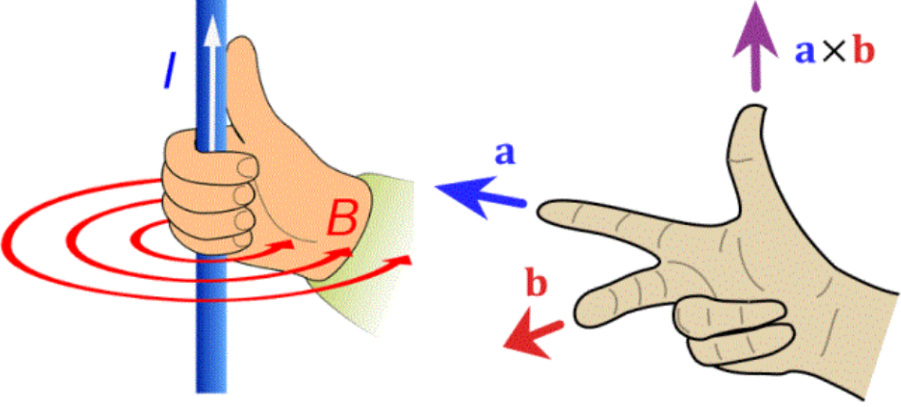
\includegraphics[width=0.7\linewidth]{rhr}
	\end{center}

	This direction will be perpendicular to both the current, and the $\vec r-\vec r\prime$ vector. 
	
	\begin{mdframed}
		\textbf{Ex. } We have a solenoid with radius b and length L with N turns of tightly wound wire. This wire carries current I. We want the $\vec B$ field anywhere on the z axis. 
		\begin{center}
			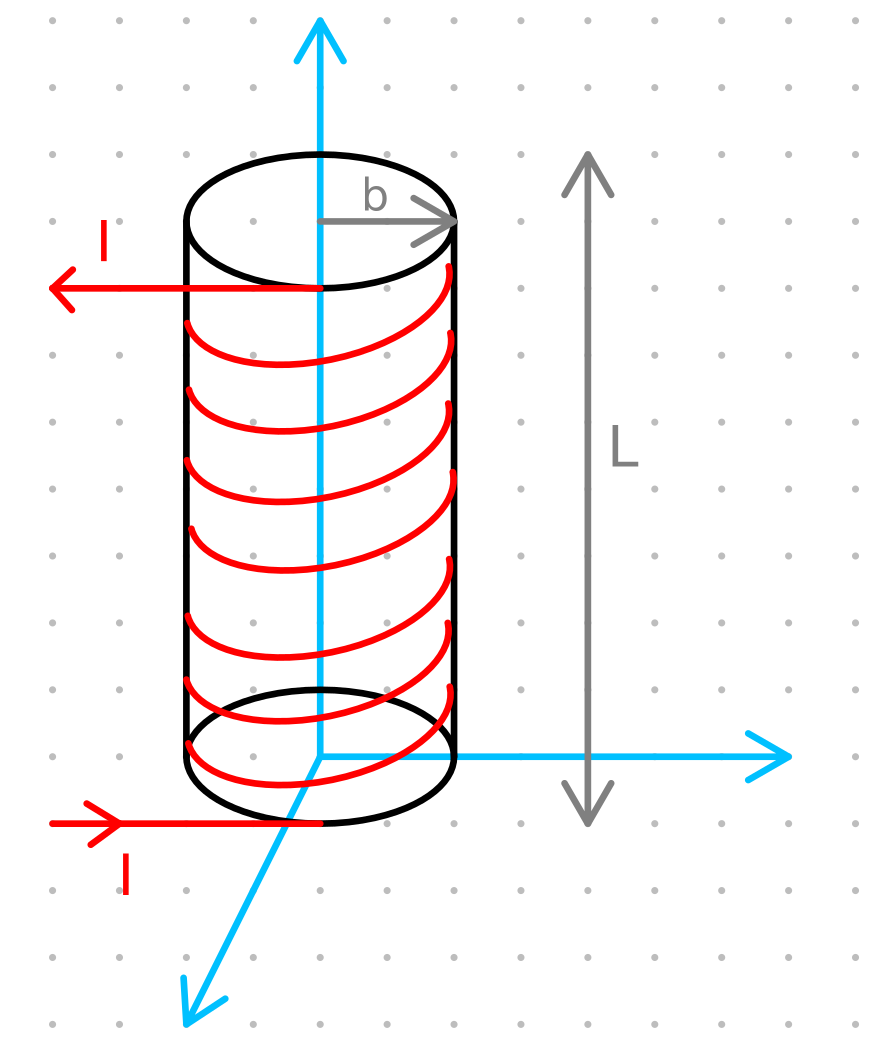
\includegraphics[width=0.34\linewidth]{ex2}
		\end{center}
		We will use the biot savart law, although we could also use Amperes law with no problem. 
		
		We need to use the 2D version of this since we have a surface of charge (the wire can be treated as a solid surface since the wire is \textbf{tightly wound})
		\begin{align*}
			\vec B = \frac{\mu_0}{4\pi}\int_{S\prime}\frac{J_s\mathrm \times (\vec r - \vec r\prime)d \vec S\prime}{|\vec r - \vec r\prime |^3} \qquad \vec r = z \hat z \qquad \vec r\prime = b\hat \rho + z\prime \hat z \qquad \mathrm d s\prime = b \mathrm d \phi \mathrm d z 
		\end{align*}
		Since the field is going in the $\rho$ direction, we use that differential surface element which is $\rho \mathrm d \phi \mathrm d z$.
		
		We also need to get $J_S$ which is just $NIL^{-1}$ in the $\hat \phi$ direction since it is the product of the number of turns, the current going through the wire, and all that divided by the length. 
		
		Then we can plug all this into the B-S equation and solve. 
		\begin{align*}
			\vec B = \frac{\mu_o}{4\pi} 
			\frac{NI}{L}\int_0^{2\pi} \int_0^{L}\frac{\hat \phi\times (z-z\prime)\hat z -b\hat\rho}{(b^2+(z+z\prime)^2)^{3/2}}\mathrm d z \mathrm d \phi
		\end{align*}
		Doing the cross prouct we get $(z-z\prime) \hat \rho + b \hat z$. Since the resulting field is only in the z direction, then $\rho$ goes to 0. 
		\begin{align*}
			\vec B = \frac{\mu_o NI b}{4\pi L}\int_0^{2\pi} \int_0^{L}\frac{\mathrm d z \mathrm d \phi}{(b^2+(z+z\prime)^2)^{3/2}} \hat z = \text{CALC}
		\end{align*}
		
	\end{mdframed}
	
	\subsection{Amperes Law}
	This is just like gausses law for electric fields in that it allows us to simplify the calculations for magnetic fields, but only under specific curcumstances. 
	
	Basically, we create an \textbf{amperian loop} (path) that when taken the dot product with the $\vec H$ field creates a nice math situation.
	\begin{align*}
		\oint \vec H \cdot \mathrm d \vec l = I_{enclosed}
	\end{align*}
	\begin{enumerate}[noitemsep]
		\item Predict Direction of $\vec H$
		\item Choose amperian path
		\item Calculate
	\end{enumerate}

	\subsection{Magnetic Flux}
	The \textbf{magnetic flux} $\Phi$ going through a surface is simply defined as:
	\begin{align*}
		\text{FLUX} = \Phi = \oint \vec B \cdot \mathrm d \vec s
	\end{align*}
	
	\begin{mdframed}
		\textbf{Ex. } We have a long straight thin wire carrying current I. We want to find the flux going through a plane with rardius going from 1m to 10m, and height going from 5m to 50m. 
		\begin{center}
			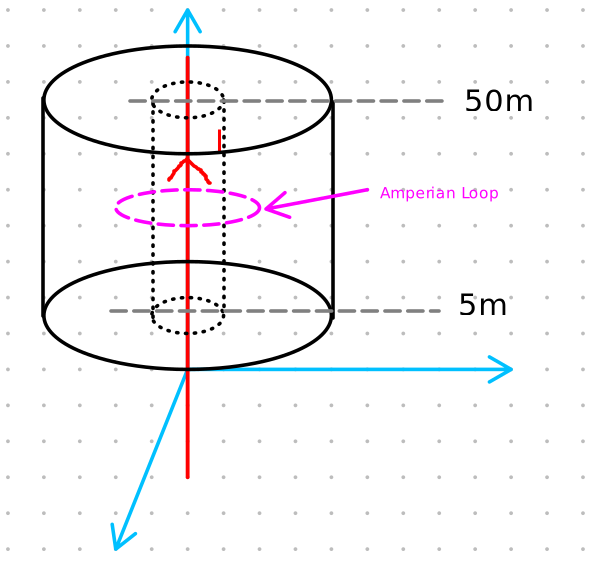
\includegraphics[width=0.4\linewidth]{ex3}
		\end{center}
		I know the flux formula is $\Phi = \oint \vec B \cdot \mathrm d \vec s$. So I need to get the magnetic field $\vec B$. Since the flux is just through the surface, it will be $\mathrm d \rho \mathrm d z$.

		I will use Amperes Law to find the B field with an amperian loop around the current wire. 
		\begin{align*}
			\int \vec H \mathrm d l = I_{enc} \implies \int \vec B \mathrm d l = I_{enc} \mu_o \implies H_\phi \hat \phi \cdot 2\pi \rho = I\mu_o \implies \vec H = H_\phi = \frac{I\mu_o}{2\pi \rho} \hat \phi
		\end{align*}
		Now I need to get the flux:
		\begin{align*}
			\Phi = \oint \vec B \cdot \mathrm d \vec s = \int_1^{10}\int_5^{50} \frac{I\mu_o \hat \phi \cdot \mathrm d\rho \mathrm d z \hat\phi}{2\pi\rho} = \frac{I\mu_o}{2\pi}\int_1^{10}\int_5^{50}\frac{\mathrm d \rho \mathrm d z}{\rho} = \text{CALC}
		\end{align*}
		
	\end{mdframed}

	\subsection{Magnetic Forces}
	We say that the magnetic force produced by \textbf{a wire} $1$ on \textbf{another wire} $2$ is: 
	\begin{align*}
		\vec F_2 = \int I_2\mathrm d \vec l_2 \times \vec B_1
	\end{align*}
	So basically we need to get $\vec B$ using probably amperes law, and then assuming we know I, we can calculate the magnetic force $\vec F_m$.
	
	\begin{mdframed}
		\textbf{Ex. }
	\end{mdframed}
	
	\subsection{Torques}
	The torque caused on a magnetic field uses the \textbf{magnetic dipole moment} $\vec m$.
	\begin{align*}
		\vec m = I\int \mathrm d \vec s = IA\hat n
	\end{align*}
	This is in the direction \textbf{perpendicular to the surface}. Hence why it is a normal vector ($\hat n$).
	\begin{align*}
		\vec \tau = \vec m \times \vec B
	\end{align*}
	The torque $\vec \tau$ is just the cross product between the magnetic field and the magnetic dipole moment vectors.
	
	\begin{mdframed}
		\textbf{Ex. }
	\end{mdframed}
	
	\subsection{Boundary Conditions}
	This is the same idea as boundary conditions for elecctric fields. If we have 2 magnetic fields at a boundary, we split it up into \textbf{normal and tangential components}. Then we apply the following conditions:
	\begin{align*}
		&B_{n1} = B_{n2} &H_{t1} - H_{t2} = J_s
	\end{align*}
	Note that $H = \frac{B}{\mu}$ and often $\mu_1 \ne \mu_2$. Also, often $J_S=0$ which means $H_{t1} = H_{t2}$
	
	\begin{mdframed}
		This is very similar to boundary conditions in Electric Fields, so an example can be found in that section.
	\end{mdframed}
	
	\section{Dynamic Currents}
	This section is about \textbf{changing currents}. These are currents that vary with time. 
	
	\subsection{EMF}
	We call $\epsilon$ the Electromotive Force (EMF) which is not actually a force, but a \textbf{voltage} measured in volts. It is caused by motion in a field. 
	\begin{align*}
		&\epsilon = \int(\vec v \times \vec B)\cdot \mathrm d \vec l = -\frac{\mathrm d \Phi}{\mathrm d t} &\text{ Faraday's Law}
	\end{align*}
	Basically if we know the velocity and $\vec B$ field, we can find the EMF, or if we know the magnetic flux $\Phi$, we can derive it with respect to time and get the EMF. 
	
	The reason for the negative in front of the derivative is that the \textbf{direction of the induced current} will oppose the \textbf{change in magnetic flux}. This is known as Lenz's law.
	
	\begin{mdframed}
		\textbf{Ex. } Using Lenz's law we can find the direction of the induced current.
		
		Recall that $\otimes$ means going INTO the page, and $\odot$ means going OUT of the page.
		
		\begin{center}
			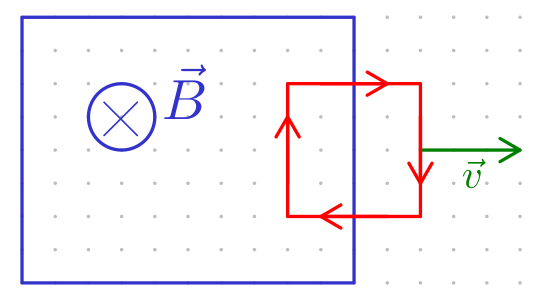
\includegraphics[width=0.3\linewidth]{lenz1}
		\end{center}
		Here $\vec B$ is decreasing ($\Delta \vec B$ is therefore coming OUT of the page $\odot$) which means that the induced current will go in a direction that is INTO the page $\oplus$. Using the right hand rule, we get that a $\vec B$ going INTO the page means current going clockwise.
		
		The reason $\vec B$ is decreasing is because $\vec v$ is pulling the current out of the $\vec B$ field, reducing the area and therfore reducing the strength of $\vec B$ going through the current loop.
		
		\begin{center}
			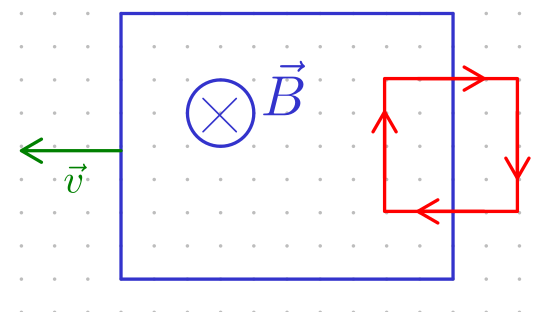
\includegraphics[width=0.3\linewidth]{lenz2}
		\end{center}
		Here $\vec B$ is also decreasing, which means that $\Delta \vec B$ is $\odot$, and therfore the induced current will be $\otimes$ creating a clockwise current.
		
		\begin{center}
			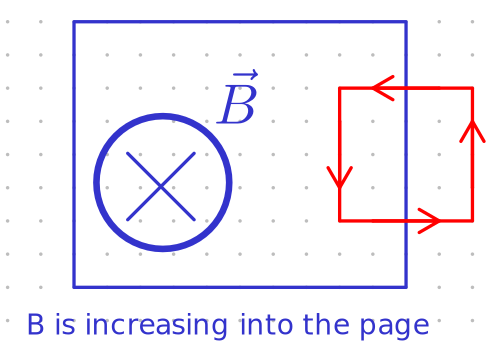
\includegraphics[width=0.3\linewidth]{lenz3}
		\end{center}
		Here $\vec B$ is increasing $\otimes$ which means $\Delta \vec B$ is $\otimes$. So the induced current will be $\odot$ creating a counter clockwise current.
		
	\end{mdframed}

	\begin{mdframed}
		\textbf{Ex. }
	\end{mdframed}
	
	
\end{document}